
% !TeX spellcheck = en_GB
\documentclass[12pt]{article}
\usepackage[utf8]{inputenc}
\usepackage{url}
\usepackage{amsmath}
\usepackage[russian,english]{babel}
\usepackage{hyperref}
\usepackage{color}
\usepackage[dvipsnames]{xcolor}
%\definecolor{cbrred}{rgb}{0.93, 0.066, 0.2}



\usepackage{rotating}

\usepackage{float}
\definecolor{newred}{RGB}{144,50,50}
\definecolor{cbrred}{rgb}{0.93, 0.066, 0.2}

\hypersetup{
	colorlinks=true,
	linkcolor=blue,
	filecolor=magenta,
	urlcolor=blue,
	citecolor=newred
}

\usepackage{sectsty}
\sectionfont{\color{cbrred}}
\subsectionfont{\color{cbrred}}
\subsubsectionfont{\color{cbrred}}



\usepackage{listings}
\usepackage{longtable}

\usepackage[a4paper, margin=1in]{geometry}

\usepackage[T1,T2A]{fontenc}
\usepackage{fontspec}
\setmainfont[Ligatures=TeX]{arial.ttf}


%\usepackage{helvet}
%\renewcommand{\familydefault}{\sfdefault}



\usepackage{caption}
\usepackage{subcaption}
% \usepackage{pscyr}

\usepackage{csquotes}
\usepackage{graphicx}
\usepackage{caption}
\usepackage{subcaption}
\usepackage{enumerate}
\usepackage[usestackEOL]{stackengine}
\usepackage{adjustbox}
\usepackage{morefloats}
\usepackage{tikz,forest}
\usetikzlibrary{arrows.meta}
\usepackage[doublespacing]{setspace}
\usepackage[numbered,framed]{matlab-prettifier}

\usepackage{pdfpages}


\usepackage[sort]{natbib}
\newcommand\SingleChartWidth{0.7}

% these set the VTB Cap format
\newcommand{\localtextbulletone}{{\raisebox{.45ex}{\rule{.6ex}{.6ex}}}}
\renewcommand{\labelitemi}{\localtextbulletone}

\usepackage{fancyhdr}
\pagestyle{fancy}
\setlength{\abovedisplayskip}{0pt}
\setlength{\belowdisplayskip}{0pt}
% \rhead{\includegraphics[width=4cm]{vtbcapitallogo.png}}


%\usepackage{exsheets}
%\usepackage{tasks}
%\SetupExSheets{counter-format=qu[A]:}
%http://ctan.math.washington.edu/tex-archive/macros/latex/contrib/exsheets/exsheets_en.pdf


\graphicspath{{"G:/Research/Economy&strategy/iav/macrodata/emf/"}}

\title{Macroeconomic archaeology and replication}

\author{
	Isakov, Alex PhD \\
	\texttt{alex.isakov@vtbcapital.com}
	\and
	Khazanov, Alexey \\
	\texttt{khazanov@bc.edu}
	\and
	Orlov, Andrey \\
	\texttt{orlovad@cbr.ru}
	\and 
	Borodin, Alexander \\
	\texttt{alexander.d.borodin@gmail.com}
}

\date{\today}

\begin{document}
	
\maketitle
	
\begin{abstract}

The dominating approach to research distribution is a mixture of modern and ancient: while empirical methods tend to be advanced, the disclosure of methodology is typically very limited, hardly allowing a reader to trace the path from data to conclusions. We believe this is a root cause of two crises: the replication crisis and the stagnation of knowledge spreading. In this note we diagnose the limits to disclosure of the results. We then provide a sketch of what we would consider a more appropriate level of disclosure by attempting to reproduce a model that we believe to eventually evolve into one of the CBR's core analytical tools. Challenges we meet in this exercise inform our recommendations for communication of the research on monetary policy and in economics more generally. 
\end{abstract}

\newpage 
\tableofcontents
\newpage 
\section{Monetary policy and accumulation of knowledge}

\section{Introduction}

Progress and advances in the economic policy conduct largely depend on how well the production and accumulation of knowledge are organised. This knowledge is typically synthesised from history and experience. 

Although in many cases the policy rule itself becomes the subject of debate (e.g., \cite{belongia2016evolution}), at the modern stage the textual material generated by the policy makers is relatively abundant ({\it e.g.}, speeches, policy documents). At the same time, the knowledge regarding the tools policy makers rely on is more scarce and sketchy. 

Taking monetary policy as an example, the opacity of the analytical toolkit means that communication between the central bank and the public may be limited. Even more importantly, in the absence of wider discussion, the development of the toolkit can be severely lagging behind the cutting edge practices at the leading central banks, in academia or in private sector. This could undermine the trust in the ability of the central banks to provide forecasts and economic analysis at the high-quality level, and, consequently, in the success of implementation of inflation targeting or another policy regime. 

This issue is by no means unique to the monetary policy or even economic policy in general for that matter, but, we believe, is one facet of the ``replication crisis'' in social sciences (see \cite{ozier2019}, among many others). 

The goal of this paper is to contribute to the history of monetary policy in Russia. We do this by addressing two issues. 

First, we attempt to run an express-test to diagnose the reproducibility of the published research in the monetary policy field in the Russian Journal of Money \& Finance (RJMF), which is a journal hosted by the Bank of Russia that invites the submissions related to the following topics: ``monetary economics including monetary policy; financial markets; banking; FinTech and Big Data in economics and finance.'' (\href{https://rjmf.econs.online/en/about/}{https://rjmf.econs.online/en/about/}). In \autoref{sec:reprisk} we find that only for 1 out of 5 published empirical studies the replication code or data can be obtained. This compares with roughly 1 out of 3 for the global benchmark studies, i.e. \cite{gertler2018make}.

Secondly, in  Section \ref{sec:ecxarche} we offer an attempt to reconstruct a working prototype of a model which eventually, according to \cite{bankofrussiampr201501}, developed into one of the CBR's core analytical tools---the Quarterly Projection Model (QPM)---based on the publicly available sources.

We stress that our goal in this part of the paper is not the {\it advancement} of the modelling techniques, but rather the {\it archaeology}, i.e. an attempt to {\it reassemble} a working model from scarce, potentially deliberately so, publicly available information. We also hope that it might serve an {\it educational purpose}---as a working example of building a QPM-type semi-structural model using the IRIS Toolbox. 

We also stress that the discussion of our replication attempt is just that - the discussion of challenges of recovering complete results from a medium that represents them incompletely. We do not attempt to offer a discussion of short-comings of a a particular model or any class of models, which are available elsewhere.

% The last section \ref{sec:conclusion} concludes. 

\section{Replication risk: the case of Journal of Money and Finance}
\label{sec:reprisk}
\subsection{Replication and research}

While the process of research, i.e. the production of new knowledge, is hard, the replication of its published results, tends to be challenging as well. For instance, in \cite{gertler2018make} the authors report that out of more than 200 the empirical economic studies they found only 16\% that had both raw data and usable code that they were able to run.  \cite{ioannidis2017power} conclude that \textquote{nearly 80\% of the reported effects in these empirical economics literature are exaggerated; typically, by a factor of two and with one-third inflated by a factor of four or more}.

Weak reproducibility and challenges of replication are socially costly: 
\begin{itemize}
    \item they limit the use of research results in policy conduct because of the concerns related to their robustness;
    \item they limit the spillovers of knowledge (and what other goal in principle does the publication in a journal have?) and ability to learn applied research skills from published articles by fellow researchers and students;
    \item they slow down the development of the research agenda, because of the, requiring researchers to replicate the results from scratch despite the technical complexity of their empirical approach;  %  // complicated nature of the incremental technical improvement
    \item they impede other researchers' ability to check and confirm results independently.
\end{itemize}

The last effect is potentially built in by institutional design of the academy, as noted in \cite{gertler2018make}, as incentives of those who produce novel results and those who replicate them are in conflict: journals tend to accept papers which refute previously published results more readily then those confirming them. 

The response of the the academic community to the replication crisis has been along two lines.

First, projects such as Macro Model Database (\href{https://www.macromodelbase.com/}{https://www.macromodelbase.com/}) and Replication Wiki  (\href{http://replication.uni-goettingen.de/}{httpshttp://replication.uni-goettingen.de/}) sprung up to coordinate efforts in verification of the existing results. % the Repr

Second, a new class of studies--- studies of the other studies or  {\it meta-studies}, emerged. These studies which survey the academic  journals' websites to understand how pervasive are requirements to publish original data and codes, how frequently these are available. They can also focus on the  replication of published results and on studying possible biases in the body of published work. 

Third, the research community started to discuss more actively the institutional changes that can be introduced to create incentives for researchers to produce results which are more robust and more easily verifiable, the best ways to harmonise incentives of researchers and reproducers, and ultimately align incentives of the academia and the public.

The practice of verification has a long history in economic research, as shown by \cite{christensen2018transparency}: \textquote{Feldstein (1974) estimates a life cycle model showing that social security reduces private savings by as much as
50\%. [...] but Leimer and Lesnoy (1982) discovered that a flaw in Feldstein’s computer program that overestimated the growth rate of Social Security wealth for widows led to larger effects of Social Security wealth than when the mistake was corrected.}

However, we claim that the practice of posting data and code remains fully foreign to the universe of Russian economic academic journals. But could it be that the cooperation between researchers is not inhibited by this lack of infrastructure, and the tools are freely shared through other channels?

Below we suggest an approach to illustrating the gravity of the replication crisis under the present conditions. 

\subsection{Replication in harsher climates}

First, we are not aware of the existence of a top-tier Russian economic journal that systematically publishes underlying data or codes to accompany an article, as it is done by American Economic Association journals that are considered as one of the most reputable in the profession\footnote{See Data and Code Availability Policy at American Economic Review's website:
\href{https://www.aeaweb.org/journals/policies/data-code}{https://www.aeaweb.org/journals/policies/data-code}}.

We thus cannot follow in the footsteps of \cite{gertler2018make}, who collect code and data directly from the journals' websites. 

Instead in order to assess the reproducibility of research we conducted the following experiment: 
\begin{enumerate}
    \item We compiled a list of all empirical articles published on the CBR's \href{https://rjmf.econs.online/}{Money and finance} journal since its relaunch, which in our case meant from issue 1 of 2018 to issue 2 of 2019. This resulted in the total of 27 articles, for full list see appendix \ref{ssec:rjmfempar}.
    \item We then emailed each of the authors requesting a replication package: data and codes behind the published results. We have introduced ourselves as a fictional graduate student {\it Anastasia Ivanova}, who was kindly asking for codes in order to learn the techniques used in the paper. Our templates for requests in Russian and English are available in the Appendix \ref{ssec:reppackreq}.
\end{enumerate}

More precisely, the algorithm was as follows: 
\begin{itemize}
    \item request started from the most recent issues of the RJMF;
	\item we mailed an author only once: if he or she succeeded in authoring a number of papers in the RJMF then we requested the replication package only for the most recent one;
	\item we emailed all the co-authors for whom the emails we made available; 
	\item we chose to address authors in English if at least one of the co-authors was affiliated with a foreign institution;
	\item we distributed our emails on Monday July 22, 2019.
	\item we established a cut off for the collection of responses on Friday August 23, 2019.
\end{itemize}

\subsection{Resum\'{e} of replies}

We identified 26 articles published in the RJMF as empirical studies. In order to query an author only once we had to censor out 4 articles, we also had to exclude another article for the lack of publicly available email address. This makes a total of {\bf 21 emails} sent out. 

In response we have received {\bf 11 replies, a 52\% gross response rate}. 

Out of the 11 replies {\bf 7 refused} to provide either data, or code which would allow replication, {\bf 4 provided both data and code} suitable for running a replication, which is a {\bf 19\% total positive response} rate. 

The causes for refusal or failure to provide the data or code were as follows:

\begin{itemize}
    \item in 2 cases the code and data have been either lost or kept by a co-author, who could not have been accessed at the time;
    \item in 2 cases part of the data was not public (neither code, nor data were provided);
    \item in 2 cases the fact that the code behind the published work is considered property of the researchers'  employer was stated as the reason for inability to share it (both of our correspondents claimed that it can be potentially recovered from one or several publicly available sources);
    \item in 1 case the researcher only inquired regarding institutional affiliation and did not return the reply. 
\end{itemize}

We have also attached two attributes to the review articles: i) whether one of the co-authors has been affiliated with the CBR (at the moment of our replication package request), ii) whether one of the co-authors was primarily affiliated with international or domestic institution.

Based on this the break-down of the response rates has been as follows: 

\begin{itemize}
    \item 2 of the positive responses came from the CBR-affiliated authors, which means a 40\% response rate (2/5), vs 12.5\% (2/16) response rate from authors not affiliated with the CBR;
    \item 3 Russian-only author groups provided data and code which means a 25\% (3/12) response rate vs 11\% (1/9) response rate from international co-authors. 
\end{itemize}

We are conscious regarding the limited scale of our sample and thus reserved regarding the conclusions that can be drawn based on it. 

And yet the small sample size itself is indicative of the gravity of the problem: roughly only 1 in 5 empirical research papers can be backed by the code and data which allow for independent verification. We believe that this response rate actually overstates what can be expected from a broader sample of Russian academic journals based on two pieces of evidence:

\begin{itemize}
    \item As we show above, response rates from non-CBR affiliated researchers tends to be lower, and we believe that the ``home bias'' of the RJMF means that they are much less concentrated in other journals;
    \item RJMF's prestigious status means that the competition for publication is higher and we believe that this competition is associated with higher willingness to provide replication materials.
\end{itemize}

\cite{hamermesh2007replication} reports: \textquote{Pure replication depends on the availability of all the information from the project that is to be replicated. Its potential importance was demonstrated to the profession in the mid-1980s by a project undertaken by the editor of the Journal of Money, Credit and Banking (Dewald et al, 1986). He sought data sets and documentation from authors of recently published and accepted
manuscripts from his Journal, received them from a disturbingly small fraction (about one-third) [...]}.

This one-third was disturbing enough for the American Economic Review to mandate that \textquote{authors of accepted articles pledge to make their data sets available upon request
unless the data were proprietary}.

We hope that, despite the smaller sample size of this study, our results will appear to be disturbing enough to trigger similar changes in the universe of Russian economic journals. We provide the summary of our suggestions in this regard in the next subsection.



\subsection{A way forward}

The results we obtained in the exercise about rise a question---what can be done to improve the situation from the {\it institutional} point of view? We would like to share our opinion regarding the way forward. In large part it is informed by the work we have done for this paper and is line with \cite{hamermesh2007replication} noting: \textquote{Any demand for replication must arise from the profession as a whole, as intermediated by the actions and decisions of the editors of the most visible professional journals.}

We believe that a change in the quality of the monetary policy related research requires rethinking of the role of the editor of the RJMF: instead of passive role of filtering the incoming submissions, we believe, the editor may take on an active role of {\it demanding } the replicability from the submitted articles, as well as {\it verifying} it.  

The procedure might be quiet simple: subjects for replication may be chosen at random among previously published results with probability distributed uniformly or, perhaps, proportional to the level of the public interest to the results (e.g., proxied by the number of downloads). 

Another change we hope to see is the change in the submission requirements making publication of data (when there are no legal restrictions) and code (always) on the designated resource. Additionally, the editors can state their preferences for research based on the publicly available data, all else being equal. 

Lastly, the journal should become an institution responsible for storing the data and code accompanying published research. One way to do that could be creation of special a repository administered by the RJMF (for instance, a popular platform used for such purposes currently is GitHub, but RJMF can as well post the data on the website).  In this way RJMF's editorial board would be able to guarantee that there would be no ``sweeping under the rug'' post publication in case if typos are discovered, and all the changes in the contents would be publicly announced. It would also guarantee the 24/7 availability of the codes, which would protect interested researchers from delays in replies to the code requests addressed personally to the authors.


In the next section we provide a case study that illustrates the the challenges of replication in case when code and data are unavailable. We also show potential set-backs in development of a highly relevant monetary policy tool this unavailability may cause. 


\section{The central bank archaeology: CBR's QPM}
\label{sec:ecxarche}

While generally researchers, in our experience, support higher standards of transparency, on the individual basis one rarely enjoys those strict standards being applied to their own results. As \cite{hamermesh2007replication} notes:
\textquote{Our expressions of preference are cheap talk. The profession provides few incentives for most active economists to produce replications of others’ research [...]}.

In this section we attempt to provide what we believe to be a useful {\it template} for sharing empirical results of monetary policy-related studies. This means providing ready access to underlying data, data transformation and estimation code, which itself is readable and closely corresponds to  the notation of the paper. 

Due to the same shortcomings of the current knowledge accumulation infrastructure in Russia, which required our mail-based exercises in the previous section---no journal in Russia currently systematically publishes neither code nor data---we will opt for a bit of macroeconomic archaeology, i.e. reconstructing research solely from published articles' text, instead of rerunning publicly  available original codes (defined as ``pure verification'' in  \cite{hamermesh2007replication}). 

To draw further analogy with archaeology and history, we can roughly say that the two key, or at least important, sources of our knowledge about the past, are {\it texts} and {\it tools}. Unless texts provide a detailed description of, for instance, a production method, we wouldn't be able to infer it without discovering tools employed for this process. Further, the production process can shed light on regional trade patterns, or reveal the logic behind the structure of an industry and the society. For an example, see a fascinating study by \cite{nunn2011potato}.

By analogy, we have plenty of textual evidence regarding the conduct of monetary policy that allows to draw some mnemonic rules regarding the way the central bank employs the available data to produce forecasts and monetary policy decisions. However, the tools monetary policy makers rely on that are available for our ``discovery'' are rather more obscure. 

So to partially rectify this issue as well as to provide the template for publication of the monetary policy oriented research we choose as a challenge to replicate one of the earliest available versions of CBR's Quarterly Projection Model (QPM). There are two primary reasons for our choice of the QPM for this exercises:

\begin{itemize}
    \item it appears to eventually become one of the CBR's core analytical tool. As \cite{bankofrussiampr201501} notes: \textquote{The Bank of Russia’s forecast is created through a process of reconciling expert judgement and calculations based on a set of models in a system for forecasting and analysis. The core of the system is the quarterly forecasting model (QFM).}
    \item it is yet to be published without crucial omissions (such as key parameter estimates) and in form suitable for replication.
\end{itemize}

Before proceeding with the exercise, we believe it is necessary to state our goals, and also to clarify the goals that we definitely do not attempt to achieve. We attempt to reconstruct the model based on {\bf publicly available sources} within a template, which we consider appropriate for publishing empirical work of this kind. 

We, however, do not attempt to improve upon this work, and neither do we attempt any exercises testing predictive power of the QPM. These types of efforts, we believe, should become ever so slightly easier due to this work. Current section proceeds as follows. First, in subsection \ref{ssec:pusoqpm} we review publicly available source on the structure of the QPM. Second, in subsection \ref{ssec:equqpm} we layout the equations of the QPM in the notation of the preceding literature. Third, we comment on the data used and transformation applied in subsection \ref{ssec:dataqpm}. Fourth, we describe our estimation approach in subsection \ref{ssec:estqpm}.

\subsection{QPM: Literature review}
\label{ssec:pusoqpm}

We believe that the available public information regarding the QPM is limited to three sources: \cite{bgpp2008} (BGPP), \cite{borodin2014} and \cite{bankofrussiampr201501}. We highlight that to a varying degree all of the authors were involved at some point in the development of the CBR's QPM, but out replication is derived strictly from publicly available materials.

BGPP is the main paper where the authors provide the outline of the model, estimates of a selection of its parameters and paths for equilibrium output and other indicators the model implies.

\cite{borodin2014} is a brief presentation which hints at the direction of work the CBR might have pursued since BGPP. It also illustrates the scope of phenomena which can be included in the QPM-type models. It seems like an impossible task to track all changes, but some of them can be pinned down by direct comparison to corresponding equations in the BGPP:

\begin{itemize}
    \item instead of relying on a single Phillips curve for headline inflation there are three curves for food, non-food and services inflation;
    \item for output gap, the effects of the deviation of the market rate and real exchange rate from their equilibrium levels have been combined into an aggregate named $rmci_t$, which likely stands for real monetary conditions index;
    \item domestic output gap is now a function of the lagged foreign gap instead of its contemporaneous value;
    \item for all the core equations the future value of inflation $\pi{4}_{t+4}$ has been substituted with its expected value, which might mean that this operator of expectations might contain a backward-looking element; 
    \item the model explicitly account for the terms of trade (which are important for equilibrium paths of the real exchange rate and output) and the Balassa-Samuelson effect (affects relative price growth for tradable and non-tradable parts of CPI).
\end{itemize}

\cite{bankofrussiampr201501} does not provide new insights into the structure of the model or its further development, but highlights its core role in the CBR's analytical toolkit. At this point we believe, that the version of the model referred to is, we believe, a different version of the QPM then one presented in the BGPP.

Below we will focus on the QPM version provided by the BGPP, and will not account for the improvements introduced later. This is in line with our goal of providing the template and reconstructing the original version of the tool. 

\subsection{QPM: Model outline}
\label{ssec:equqpm}

For ease of exposition, in the model outline below we follow the structure of the BGPP. The subsections also contain links to corresponding appendices, where the code is outlined. We build the mode using the IRIS Toolbox\footnote{IRIS Toolbox can be found here: \href{https://github.com/IRIS-Solutions-Team/IRIS-Toolbox/wiki/IRIS-Macroeconomic-Modeling-Toolbox}{https://github.com/IRIS-Solutions-Team/IRIS-Toolbox/wiki/IRIS-Macroeconomic-Modeling-Toolbox}}. Supplementary materials including the code and data are available at the GitHub \href{https://github.com/alexisakov/replica}{repository}.

\subsubsection{The key transition equations}
The BGPP's first four core equations are the Phillips curve, the investment-saving (IS) curve, the uncovered interest rate parity (UIP)  and the Taylor rule. The code is provided in Appendix \ref{ssec:qpmeq1}. 

The Phillips curve describes the evolution of inflation:

\begin{equation}
	\pi_t = \alpha_1 {\pi}4_{t+4} + \alpha_2{\pi}4_{t-1} + (1-\alpha_1-\alpha_2)*(\Delta ls_t + \pi{_t}^{for}-\Delta lz_{t}^{eq}) + \alpha_3 y_{t}^{gap}+\varepsilon_{t}^{(1)}
\end{equation}

The IS curve describes the evolution of the output gap:

\begin{equation}
	y_{t}^{gap} = \beta_1 y_{t+1}^{gap} + \beta_2 y_{t-1}^{gap} - \beta_3(rr_{t-1}^{market} - rr_{t-1}^{market eq}) + \beta_4*lz_{t-1}^{gap}+\beta_5 y_t^{gap for}+\varepsilon_{t}^{(2)}
\end{equation}

The uncovered interest rate parity links interest rates with expected exchange rate dynamcis:

\begin{equation}
	ls_t = \delta_1 ls_{t+1} + (1-\delta_1)*(ls_{t-1} + \Delta_2ls_t^{eq}/4) - (rs_t-rs_t^{for} - \rho_t)/4 + \varepsilon_{t}^{(3)}
\end{equation}

The Taylor-type monetary policy rule:

\begin{equation}
	rs_t = \gamma_1 rs_{t-1} + (1-\gamma_1)*(rs_{t}^{neutral} + \gamma_2 (\pi4_{t+4}-\pi_{t+4}^{tar})+\gamma_3 y_t^{gap}) + \varepsilon_{t}^{(4)}
\end{equation}

\subsubsection{Exogenous variables transition equations}

Next block defines the exogenous equations, which are typically defined as random walks or auto-regressions. The code is provided in the appendix \ref{ssec:qpmeq2}. 

Inflation target: 

\begin{equation}
	\pi_t^{tar} = \pi_{t-1}^{tar} + \eta_t^{(1)}
\end{equation}

Equilibrium output growth:

\begin{equation}
	\Delta y^{eq}_t = \chi y^{eq}_{t-1} + (1-\chi)*\Delta y^{eq}_{ss} + \eta_t^{(2)}
\end{equation}

Nominal interest rate on bank lending:

\begin{equation}
	rs^{market}_t = \xi rs^{market}_{t-1}  + (1-\xi) * ((rs_t+rs_{t+1}+rs_{t+2}+rs_{t+3})/4+\rho_t^{market}) + \eta_t^{(3)}
\end{equation}

Equilibrium nominal interest rate on bank lending:

\begin{equation}
rr^{market~eq}_t = \zeta_2 rr^{market~eq}_{t-1}  + (1-\zeta_2) * rr^{market eq}_{ss} + \eta_t^{(4)}
\end{equation}

Term premium:

\begin{equation}
	\rho^{market}_t = \kappa \rho^{market}_{t-1}  + (1-\kappa) * \rho^{market}_{ss} + \eta_t^{(5)}
\end{equation}

Equilibrium change of the real exchange rate:

\begin{equation}
	\Delta lz_t^{eq} = \zeta_1 \Delta lz_{t-1}^{eq} + (1-\zeta_1) \Delta lz_{ss}^{eq} + \eta_t^{(6)}
\end{equation}

Risk premium:

\begin{equation}
	\rho_t = \zeta_3 \rho_{t-1}  + (1-\zeta_3) * \rho_{ss} + \eta_t^{(7)} 
\end{equation}

Foreign output gap:

\begin{equation}
	y^{gap~for}_t = 0.85 y^{gap~for}_{t-1} + \eta_t^{(8)}
\end{equation}

Foreign nominal interest rate:

\begin{equation}
	rs^{for}_t = 0.85 rs^{for}_{t-1} + \eta_t^{(9)}
\end{equation}

Foreign inflation:

\begin{equation}
	\pi^{for}_t = 0.85 \pi^{for}_{t-1} + \eta_t^{(10)}
\end{equation}

\subsubsection{Identities}

This block contains definitions of variables, which are some algebraic transformations of other variables and do not have their own shocks. The code is provided in the appendix \ref{ssec:qpmeq3}. 

Annual inflation:

\begin{equation}
	{\pi}4_t = (\pi_t + \pi_{t-1} + \pi_{t-2} + \pi_{t-3} ) / 4
\end{equation}

Output:

\begin{equation}
	y_t = y_t^{eq} + y_t^{gap}
\end{equation}

Equilibrium output:

\begin{equation}
	y_t^eq = y_{t-1}^eq + \Delta y_t^eq / 4
\end{equation}

Nominal neutral policy rate:

\begin{equation}
	rs_t^{neutral} = rr_t^{market~eq} - \rho_t^{market} + {\pi}4_{t+4}
\end{equation}

Real policy rate 

\begin{equation}
	rr_t = rs_t - \pi_{t+1}
\end{equation}

Real bank interest rate: 

\begin{equation}
	rr_t^{market} = rs_t^{market} - {\pi}4_{t+4}
\end{equation}

Nominal Exchange rate dynamics:

\begin{equation}
	\Delta ls_t = 4 (ls_t - ls_{t-1})
\end{equation}

Equilibrium exchange rate change over two quarters: 
\begin{equation}
	\Delta_2 ls_t^{eq} = \pi_t - \pi_{t+1} - \pi_t^{for} - \pi_{t+1}^{for} + 2 \Delta lz_t^{eq}
\end{equation}

Real exchange rate level:
\begin{equation}
	lz_t = lz_{t-1} + (\Delta ls_t -\pi_t + \pi_t^{for})/4
\end{equation}

Equilibrium real exchange rate level:
\begin{equation}
	lz_t^{eq} = lz_{t-1}^{eq} + \Delta lz_{t}^{eq}/4
\end{equation}

Real exchange rate gap: 
\begin{equation}
	lz_t^{gap} = lz_t - lz_t^{eq}
\end{equation}

Foreign real interest rate:
\begin{equation}
	rr_t^{for} = rs_t^{for} - \pi_{t+1}^{for}
\end{equation}

\subsection{The data and transformations \label{ssec:dataqpm}}


The observed part of the model includes the following macroeconomic variables: 1. Interest rates:  (a) domestic policy rate or money market rate; (b) domestic bank lending interest rate; (c) country risk premium; (d) foreign policy or money market rate. 2. Inflation rates: (a) domestic CPI level; (b) foreign CPI level 3. Economic activity levels: (a) domestic output gap; (b) foreign output gap.  4. Exchange rate. 

The IRIS code for linking the model variables to the data is provided in Appendix \ref{ssec:qpmeq4} {\color{blue} and is available at the GitHub repository \href{https://github.com/alexisakov/replica}{https://github.com/alexisakov/replica}}  Below we describe the data used and transformations applied. For the complete code of the data transformations, see Appendix \ref{ssec:qpmeq5}. 

\begin{table}[H]
\centering
\resizebox{\textwidth}{!}{\begin{tabular}{llllll}
 & Variable & Observed & Transformations \\ \hline \hline
\textbf{Interest rates}  & & \\
domestic money market rate & $rs$ & MIACR, o/n & fq,log \\
domestic bank lending rate & $rs^{market}$ & corporate, up to 1yr & fq,log \\
country risk premium & $\rho$ & CDS,5yr & fq,log \\
foreign money market rate & $rs^{for}$ & EFFR, o/n & fq,log \\
\textbf{Inflation rates} & &\\
domestic CPI level & $\pi$ & CPI & fq, sa, log, diff \\
foreign CPI level & $\pi_f$ & CPI & fq, sa, log, diff  \\
\textbf{Economic activity} & & & \\
domestic output &  $y$ & GDP SA & log \\
foreign output gap  & $y^{for~gap}$ & GDP & HP,log  \\
\textbf{Exchange rate} & $ls$ & USDRUB & fq,log  
\end{tabular}}
\end{table}

Legend: fq - frequency transformation, which here means down-sampling daily and monthly data to model's quarterly frequency, log - natural log transformation, HP - Hodrick-Prescott filtered gap, sa - seasonal adjustment with ARIMA-X12-SEATS. 

\subsection{Parameterisation}
\label{ssec:estqpm}

The model contains a total of 23 parameters, while the BGPP offers calibration for 8 of them. We then have to estimate the remaining 15. 

There are broadly two estimation approaches available to us:
\begin{enumerate}
    \item {\bf estimation}---attempt to fit the remaining parameters to the data as closely as possible assigning them some prior distributions;
    \item {\bf calibration}---manually set the parameters at the values which produce impulse responses consistent with our expectations and broad theory. 
\end{enumerate}

We attempt to use both approaches. 

\subsection{Estimation}

We estimate the model by assigning prior distribution to parameters. The priors are available in the table below, where we provide the details on the approach to estimation: BGPP means that the parameter estimate is provided by the original paper, while for the remaining parameters we offer our priors used in estimation. 

The code for estimation is available in \autoref{ssec:qpmeq6}.

\subsection{Calibration}

The BGPP version of the model, as is typical when the data is scarce, was calibrated rather than estimated, see \cite{borodin2014}. As not all the coefficients are reported in the note, we attempt to complete the model by calibrating the remaining parameters. 

In this calibration we following these general principles regarding the intended effects of the following shocks: 

\begin{itemize}
    \item demand shock
\begin{itemize}
    \item output gap increases by 1pp or even slightly more and undershoots on the way down;
    \item inflation accelerates, but less than the size of the shock, then converges back to the target rate in 2-3 years, it may also slightly undershoot the target;
    \item interest rate increases more than inflation (i.e. the real interest rate also goes up), but then descends to the neutral rate, yet  initially the real rate may decrease due to monetary policy inertia typical for 00's;
    \item FX initially may appreciate, but later settles lower than the original level;
    \item real FX rate gap remains negative from the start, but may overshoot later;
\end{itemize}
\item cost-push/supply shock 
\begin{itemize}
    \item inflation initially gains more than the shock, due to persistent inflation expectations;
    \item interest rates react less than to the demand shock (real interest rate gains less or even remain flat)
    \item output gap becomes negative, but less in scale than the shock size;
    \item real exchange rate is negative, appreciating fast;
\end{itemize}
\item interest rate/monetary policy shock
\begin{itemize}
    \item exchange rate appreciates, negative exchange rate gap, negative output gap;
    \item interest rate gradually returns back to equilibrium and key variables follow.
\end{itemize}
\item inflation target shock: as the target is defined as random walk (more on that in the section below) then its shocks are basically permanent shifts in the price level. Say, with the decrease in the inflation target the model is expected to display lower interest rates, decline in inflation expectations (however this may be less strictly so if the credibility of the monetary policy remains contested).
\item FX shock: is similar to the demand side shock.
\end{itemize}

\begin{table}[!htbp]
\centering

\resizebox{\textwidth}{!}{\begin{tabular}{lcclcccc}
   & Equation & Parameter & Prior  & estimated & Value: BGPP & Value: Estimated & Value: Calibrated \\ \hline \hline
1  & (1)      & $\alpha_1$ & BGPP & n & 0.45 & - & - \\
2  & (1)      & $\alpha_2$ & BGPP & n & 0.45 & - & -  \\
3  & (1)      & $\alpha_3$ & BGPP & n & 0.23 & - & -  \\
4  & (2)      & $\beta_1$ & B(2,2) & y & -   & 0.00 & 0.10 \\
5  & (2)      & $\beta_2$ & BGPP & n & 0.3   & - & -  \\
6  & (2)      & $\beta_3$ & BGPP & n & 0.1   & - & -  \\
7  & (2)      & $\beta_4$ & BGPP & n & 0.2   & - & - \\
8  & (2)      & $\beta_5$ & B(2,2) & y & -   & 0.00 & 0.50 \\
9  & (3)      & $\delta_1$ & B(2,2) & y & -  & 0.98 & 0.20  \\
10 & (4)      & $\gamma_1$ & BGPP & n & 0.4  & - & - \\
11 & (4)      & $\gamma_2$ & G(1,2) & y & -  & 0.00 & 1.50  \\
12 & (4)      & $\gamma_3$ & G(1,2) & y & -  & 0.00 & 0.8  \\
13 & (6)      & $\chi$     & B(2,2) & y & -  & 0.94 & 0.5   \\
14 & (6)      & $y^{eq}_{ss}$ & G(1,2) & y & - & 0.00 & 1.0 \\
15 & (7)      & $\xi$ & BGPP & n & 0.7  & - & - \\
16 & (8)      & $\zeta_2$  & B(2,2) & y & -  & 0.92 & 0.5 \\
17 & (8)      & $rr^{market~eq}_{ss}$ & G(1,2) & y & - & 0.00 & 1.00 \\
18 & (9)      & $\kappa$ & B(2,2) & y & - & 1.00 & 0.5 \\
19 & (9)      & $\rho^{market}_{ss}$ & G(1,2) & y & - & 0.02 & 1.0 \\
20 & (10)     & $\zeta_1$ & B(2,2) & y & - & 0.93 & 0.5 \\
21 & (10)     & $lz^{eq}_{qq~ss}$ & G(1,2) & y & - & 0.04 & 1.0 \\
22 & (11)     & $\zeta_3$ & B(2,2) & y & -  & 0.82 & 0.50 \\
23 & (11)     & $\rho_{ss}$ & G(1,2) & y & - & 1.57 & 1.0 
\end{tabular}}
\caption{Parameters of the replicated QPM model. Source: BGPP, authors' estimates}
\end{table}

Legend: BGPP - estimate from the BGPP, G(a,b) - gamma distribution, B(a,b) - beta distribution.

\subsection{Discussion}

The materials published by the CBR staff in the past allow us to restore equation-by-equation the model that the CBR used to employ for the purpose of economic analysis and forecasting. 

We would like to make three points regarding this excercise. 

First, with a total of just \href{https://scholar.google.com/scholar?cites=15691293148877343587&as_sdt=2005&sciodt=0,5&hl=en}{7} references, we believe, that the BPGG has up to now escaped the attention (and scrutiny) of the wide academic audience, that would be matching its central position in the CBR's toolbox, i.e. see \cite{bankofrussiampr201501}. 

Before highlighting some of the shortfalls, we need to emphasise that the task of constructing structural macroeconomic models for emerging markets is usually seen as an extremely complicated one, since some of the features of local economy are not of great interest to mainstream academic thought (e.g., the commodity-centered structure). Those models should be designed in a way which is the most convenient for the task of economic analysis and forecasting. For that reason they are  expected neither to represent the exhaustive description of the economy, nor to be 100\% microfounded and  follow the cutting-edge research in wide topics in economics (e.g., production networks, inequality issues). They should rather make sense from the point of view of key mechanisms affecting the macroeconomic aggregates and the central bank policy (in theory), and do a good job in forecasting. While the latter goal makes the usage of non-structural econometric and machine learning techniques tempting, the former still makes us keep track of the equations from the structural standpoint. This is the point that we address in the discussion. 

Our second concern is conceptual and is related to the inflation target. One of the usual assumptions implicitly made in the macroeconomic models is that the parameters of the model or, more broadly speaking, the model itself doesn't change over time. This assumption is used for the solution, for the impulse responses and for forecasting purposes, unless the model belongs to the class of models with time-varying parameters. In CBR QPM as presented in \cite{bgpp2008}, the target inflation $\pi_{t+4}^{tar}$ is {\it de facto} a parameter (random walk process, which in the absence of shocks just takes the initially set value), although it is presented as a variable. The model has a steady state close to zero inflation target (under our calibration). This deviation leads to the result demonstrated above--- the nominal exchange rate diverges, and becomes infinitesimally low with time (currency depreciates), which to be expected if inflation target is set at the significantly lower rate than global benchmark. See \autoref{ssec:qpmirfs} for illustration.

The principle question here is whether the model is fit for analyzing this kind of policy questions. Although technically we introduce a permanent shock to the model, {\it in fact} we are changing a parameter of the model. Since the 4\% target implemented by the Bank of Russia is predominantly derived from the international experience, it may theoretically be above or below the actual target level at which economy is in the steady state. Then, the currency should be infinitely appreciating, or infinitely depreciating. Unless we assume that the current dynamics of the Russian currency represents a free fall into the abyss, since the rouble's dynamics after the 2014 transition is consistent with the steady state inflation below current target, this part of the modelling apparatus is not fit for this policy exercise. Instead, the change in the target should be accompanied with a change in other parameters of the model, which would make this experiment a transition from one steady state to another. 

We understand however, that this assumption may be less dangerous if forecasting horizons are short and a forecaster plugs in a sensible estimate of the $\pi^{tar}$.

Third, we believe that even the fullest disclosure of the structure of the model and the set of parameters would not allow an outside observer to replicate its forecasts. One obvious reason is that a QPM-based forecast is usually conditional and the model does not provide any clues as to the choice of conditioning assumptions (be it oil price path, risk premium assumptions,  etc.). Another, more subtle point which is highlighted by the inflation target above is that forecasts are typical arrived at by iterating some initial state of the economy which is subject to judgement and is essential itself is a parameter, unknown to the outside observer. 

While in this note we addressed only the issues of one particular model, the point that we would like to make is more general: models used in policy and academic papers are complex. This compexity means that their behaviour can hide a lot of surprises, that cannot be inferred from the scarce description presented in the corresponding texts. The most effective treatment to this complexity is matching degree of transparency: publication of codes can allow both to learn useful shortcuts and methodological approaches, usually omitted in the technical descriptions in the papers, and to reveal possible bugs and typos. 

\section{Conclusion}
\label{sec:conclusion}

In this paper we attempt to highlight a major issue of replicability in Russian (in a general sense) macroeconomic research. We approached the issue from two sides: we asked the authors of the papers published in RJMF past relaunch  to provide replication materials, and we illustrated challenges of replication with the CBR's QPM based on open-access published materials. The conclusions we made are the following. 

First, we believe Russian economics research suffers from the replication issues experienced globally across social disciplines. We hope we've managed to provide sufficient evidence to trigger a sense of urgency for substantial reforms on this front. 

Second, current approach to publication of research results is a peculiar mixture of modern techniques and ancient medium. While it might be suitable for theoretical papers, empirical results can be communicated only incompletely in the standard article format. As \cite{christensen2018transparency} notes quoting another study: \textquote{An article about computational science in a scientific publication is not the scholarship itself, it is merely advertising of the scholarship. The actual scholarship is the complete software development environment and the complete set of instructions which generated the figures}. 

We hope the challenges in estimation of the QPM model show how limited is the traditional exposition of the results. 

Finally, we provided some suggestions for the improvement of the publication standards for empirical research in economics. A Russian macroeconomic journal that requests and posts upon publication the replication materials from the authors, as well as verifies the replicability of the paper, has a chance to produce a huge benefit for our research community and for the published authors themselves. That kind of journal can gain good reputation among the macroeconomic academic and policy community attracting attention of interested researchers that would like to dig deep into the empirical techniques in macroeconomics. 



\newpage 
\section{Appendix}

\subsection{RJMF: empirical articles issued, 1'18-2'19}
\label{ssec:rjmfempar}

\footnotesize
\begin{longtable}{llll}
Year & Issue & Article & code \\
\hline \hline
\endhead
2018 & 1     & \begin{tabular}[c]{@{}l@{}}Grafe, C., Grut, S., Rigon, L. (2018). Neutral Interest Rates in CEEMEA \\ — Moving in Tandem with Global Factors.\\  Russian Journal of Money and Finance, 77(1), pp. 6-25.\end{tabular} & GGR2018    \\
2018 & 1     & \begin{tabular}[c]{@{}l@{}}Ponomarenko, A., Sinyakov, A. (2018). Impact of Banking\\  Supervision on Banking System Structure: Conclusion from Agent-Based\\  Modelling. Russian Journal of Money and Finance, 77(1), pp. 26-50.\end{tabular} & PS2018     \\
2018 & 1     & \begin{tabular}[c]{@{}l@{}}Mamonov, M. (2018). Banks’ Hidden Negative Capital \\ Before and After the Senior Management Change at the Bank of Russia.\\  Russian Journal of Money and Finance, 77(1), pp. 51-70.\end{tabular} & M2018      \\
2018 & 1     & \begin{tabular}[c]{@{}l@{}}Panizza, U., Wyplosz, C. (2018). The Folk Theorem of Decreasing\\  Effectiveness of Monetary Policy: What Do the Data Say? Russian \\ Journal of Money and Finance, 77(1), pp. 71-107.\end{tabular} & PW2018     \\
2018 & 2 & \begin{tabular}[c]{@{}l@{}}Makinen, M., Solanko, L. (2018). Determinants of Bank Closures:\\  Do Levels or Changes of CAMEL Variables Matter?\\  Russian Journal of Money and Finance, v. 77(2), pp. 3-21.\end{tabular} & MK2018 \\
2018 & 2 & \begin{tabular}[c]{@{}l@{}}Ushakova, Y., Kruglova, A. (2018). Competition in Russia’s Banking \\ Sector Prior and After Supervision Police Enhancement: Conclusions Based on\\ Interest Rate Dispersion and Spread. Russian\\  Journal of Money and Finance, 77(2), pp. 22-50.\end{tabular} & UK2018 \\
2018 & 2 & \begin{tabular}[c]{@{}l@{}}Kreptsev, D., Seleznev, S. (2018). Forecasting for the Russian\\ Economy Using Small-Scale DSGE Models. Russian Journal \\ of Money and Finance, 77(2), pp. 51–67.\end{tabular} & KS2018 \\
2018 & 2     & \begin{tabular}[c]{@{}l@{}}Shulgin, A. (2018). Sterilized Interventions in the Form\\  of Foreign Currency Repos: VECM Analysis Using Russian Data.\\  Russian Journal of Money and Finance, 77(2), pp. 68-80.\end{tabular} & Shu2018 \\
2018 & 2 & \begin{tabular}[c]{@{}l@{}}Styrin, K. (2018). A Multi-Country Study of Cross-Border \\ Transmission of Monetary Policy by IBRN. Russian Journal\\  of Money and Finance, 77(2), pp. 81-94.\end{tabular} & Sty2018    \\
2018 & 3 & \begin{tabular}[c]{@{}l@{}}Gerlach-Kristen, P., Moessner, R. and Rosenblatt-Wisch, R. (2018). \\ Computing Long-Term Market Inflation Expectations for Countries\\  without Inflation Expectation Markets. Russian\\  Journal of Money and Finance, 77(3), pp. 23–48.\end{tabular} & GKMRW2018  \\
2018 & 3     & \begin{tabular}[c]{@{}l@{}}Nagy, E.E. and Tengely, V. (2018). External and Domestic Drivers\\  of Inflation: The Case Study of Hungary. Russian Journal of \\ Money and Finance, 77(3), рр. 49-64.\end{tabular} & NT2018     \\
2018 & 3     & \begin{tabular}[c]{@{}l@{}}Kartaev, P. and Luneva, I. (2018). Shaken, not Stirred: Comparing\\  the Effectiveness of Pure and Hybrid Inflation Targeting. Russian\\  Journal of Money and Finance, 77(3), рр. 65–75.\end{tabular} & KL2018 \\
2018 & 3     & \begin{tabular}[c]{@{}l@{}}Mamonov, M., Akhmetov, R., Pankova, V., Solntsev, O., Pestova,\\  A. and Deshko, A. (2018). Identification of Financial Sector \\ Optimal Depth and Structure from the Perspective of Economic \\ Growth, Macroeconomic and Financial Stability. Russian\\  Journal of Money and Finance, 77(3), рр. 89-123\end{tabular} & MAPSPD2018 \\
2018 & 4 & \begin{tabular}[c]{@{}l@{}}Antonova, D. and Vymyatnina, Y. (2018). Inflation and Population\\  Age Structure: The Case of Emerging Economies. Russian Journal\\  of Money and Finance, 77(4), pp. 3–25.\end{tabular} & AV2018 \\
2018 & 4 & \begin{tabular}[c]{@{}l@{}}Yakovleva, K. (2018). Text Mining-based Economic Activity\\  Estimation. Russian Journal of Money and Finance, 77(4),\\  pp. 26–41.\end{tabular} & Y2018 \\
2019 & 1 & \begin{tabular}[c]{@{}l@{}}Baybuza, I. (2018). Inflation Forecasting Using Machine\\  Learning Methods. Russian Journal of Money and Finance, \\ 77(4), pp. 42–59.\end{tabular} & Bay2018 \\
2019 & 1 & \begin{tabular}[c]{@{}l@{}}Styrin, K. (2019). Forecasting Inflation in Russia by Dynamic\\  Model Averaging. Russian Journal of Money and Finance, \\ 78(1), pp. 3–18.\end{tabular} & Sty2019 \\
2019 & 1 & \begin{tabular}[c]{@{}l@{}}Mikosch, H. and Solanko, L. (2019). Forecasting Quarterly\\  Russian GDP Growth with Mixed-Frequency Data. Russian\\  Journal of Money and Finance, 78(1), pp. 19–35.\end{tabular} & MS2019     \\
2019 & 1     & \begin{tabular}[c]{@{}l@{}}Marodin, F. A. and Portugal, M. S. (2019). Exchange Rate\\  Pass-Through in Brazil: А Markov Switching DSGE Estimation\\  for the Inflation Targeting Period. Russian Journal of Money\\  and Finance, 78(1), pp. 36–66.\end{tabular} & MP2019 \\
2019 & 1 & \begin{tabular}[c]{@{}l@{}}Ambriško, R. (2019). Fiscal Devaluation in a Small Open \\ Economy. Russian Journal of Money and Finance, 78(1), \\ pp. 67–88.\end{tabular} & A2019      \\
2019 & 1     & \begin{tabular}[c]{@{}l@{}}Borsuk, M. (2019). Forecasting the Net Interest Margin\\  and Loan Loss Provision Ratio of Banks in Various Economic\\  Scenarios: Evidence from Poland. Russian Journal of Money\\  and Finance, 78(1), pp. 89–106.\end{tabular} & Bor2019 \\
2019 & 2 & \begin{tabular}[c]{@{}l@{}}Charnavoki, V. (2019). International Risk-Sharing and Optimal\\  Monetary Policy in a Small Commodity-Exporting Economy.\\  Russian Journal of Money and Finance, 78(2), pp. 3–27.\end{tabular} & Cha2019    \\
2019 & 2 & \begin{tabular}[c]{@{}l@{}}Deryugina, E. and Ponomarenko, A. (2019). Determination \\ of the Current Phase of the Credit Cycle in Emerging Markets.\\  Russian Journal of Money and Finance, 78(2), pp. 28–42.\end{tabular} & DP2019 \\
2019 & 2 & \begin{tabular}[c]{@{}l@{}}Kilp, J., Anvari, V., Springfield, S. and Roberts, C. (2019). \\ The Impact of the Global Financial Safety Net on Emerging \\ Market Bond Spreads. Russian Journal of Money and Finance, \\ 78(2), pp. 43–66.\end{tabular} & KASR2019 \\
2019 & 2 & \begin{tabular}[c]{@{}l@{}}Fokin, N. and Polbin, A. (2019). Forecasting Russia's Key \\ Macroeconomic Indicators with the VAR-LASSO Model. \\ Russian Journal of Money and Finance, 78(2), pp. 67–93.\end{tabular} & FB2019 \\
2019 & 2 & \begin{tabular}[c]{@{}l@{}}Fomin, L. (2018). Do Higher Interest Rates on Loans and\\  Deposits and Advertising Spending Cuts Forecast Bank \\ Failures? Evidence from Russia. Russian Journal of \\ Money and Finance, 78(2), pp. 94–112.\end{tabular} & Fom2019
\end{longtable}

\subsection{Replication package request templates}
 \label{ssec:reppackreq}
 
The request in Russian:

\textquote{From: nastyaivanovaphd@gmail.com

To: [Authors]

Subjuct: О статье в ДиК

Добрый день!

Меня зовут Анастасия Иванова, я аспирант. 

Мне бы хотелось поблагодарить Вас за замечательную статью: [LINK]

Кроме того, я хочу  попытаться воспроизвести Ваши результаты и понять, как на практике проводятся расчеты в подобных исследованиях. 
Вы не могли бы, пожалуйста, поделиться исходным кодом и данными для этой статьи? Размер данных не представляет проблем - у меня большой dropbox :)

Заранее признательна!}

The request in English:

\textquote{From: nastyaivanovaphd@gmail.com % password is versus00!

To: [Authors]

Title: re article in CBR's Money and Finance

Good day!

I'm Anastasia Ivanova, a graduate student. 

I wanted to thank you for your very informative article: [LINK]

Also, I wanted to attempt to replicate your results and understand, how in practice such empirical work is done. 

Could I, please, ask for your codes and data, used in the article? The size of the data should not be a concern - I have a rather large dropbox limit :)

Thanks in advance!}

\subsection{QPM.mod}

\lstinputlisting[style=Matlab-editor]{bgpp/bgpp2008.mod}

\subsection{QPM: Core 4: Taylor rule, UIP, Phillips and IS curves}
\label{ssec:qpmeq1}

\lstinputlisting[style=Matlab-editor]{bgpp/bgpp2008TransitionEndogenous.mod}

\subsection{QPM: Exogenous processes}
\label{ssec:qpmeq2}

\lstinputlisting[style=Matlab-editor]{bgpp/bgpp2008TransitionExogenous.mod}

\subsection{QPM: Identities}
\label{ssec:qpmeq3}

\lstinputlisting[style=Matlab-editor]{bgpp/bgpp2008TransitionIdentities.mod}

\subsection{QPM: Observation equations}
\label{ssec:qpmeq4}

\lstinputlisting[style=Matlab-editor]{bgpp/bgpp2008Measurement.mod}

\subsection{QPM: From raw data to model data}
\label{ssec:qpmeq5}

\lstinputlisting[style=Matlab-editor]{bgpp/a01preparedata.m}

\subsection{QPM: Estimation}
\label{ssec:qpmeq6}

\lstinputlisting[style=Matlab-editor]{bgpp/a02estimate.m}

\subsection{QPM vs VAR(1): forecast precision}
\label{ssec:forecastprecision}

\begin{table}[!htbp]
    \begin{adjustbox}{width=1\linewidth}
\begin{tabular}{lllllllllllll}
QPM: relative to VAR(1) &       &       &       &       &        &        &        &        &        &        &        &        \\
CPI, \% QoQ SAAR        & 0.55  & 0.65  & 0.42  & 0.50  & 0.41   & 0.43   & 0.36   & 1.03   & 0.20   & 0.08   & 0.06   & 0.11   \\
FX, \% QoQ AR           & 3.61  & 3.39  & 2.47  & 3.23  & 3.01   & 1.68   & 1.75   & 3.62   & 0.61   & 0.36   & 0.40   & 1.58   \\
Policy rate, \%         & 0.04  & 0.07  & 0.06  & 0.07  & 0.05   & 0.04   & 0.04   & 0.03   & 0.02   & 0.01   & 0.01   & 0.01   \\
QPM, pp                 &       &       &       &       &        &        &        &        &        &        &        &        \\
CPI, \% QoQ SAAR        & 3.47  & 3.69  & 4.19  & 4.60  & 5.01   & 5.65   & 6.11   & 6.15   & 5.61   & 5.39   & 4.56   & 4.40   \\
FX, \% QoQ AR           & 20.62 & 27.06 & 26.89 & 27.53 & 28.12  & 29.01  & 30.18  & 31.10  & 31.49  & 32.72  & 34.11  & 35.88  \\
Policy rate, \%         & 2.32  & 4.02  & 5.10  & 5.87  & 6.22   & 6.37   & 6.49   & 6.58   & 6.70   & 6.81   & 6.78   & 6.73   \\
VAR(1), pp              &       &       &       &       &        &        &        &        &        &        &        &        \\
CPI, \% QoQ SAAR        & 6.30  & 5.66  & 10.07 & 9.12  & 12.29  & 12.99  & 16.81  & 6.00   & 28.47  & 65.21  & 80.54  & 39.05  \\
FX, \% QoQ AR           & 5.71  & 7.98  & 10.89 & 8.51  & 9.35   & 17.28  & 17.27  & 8.59   & 51.60  & 91.93  & 85.63  & 22.77  \\
Policy rate, \%         & 56.86 & 56.17 & 84.08 & 88.40 & 133.26 & 161.17 & 161.30 & 192.19 & 317.27 & 470.18 & 607.03 & 764.18
\end{tabular}
\end{adjustbox}
\end{table}

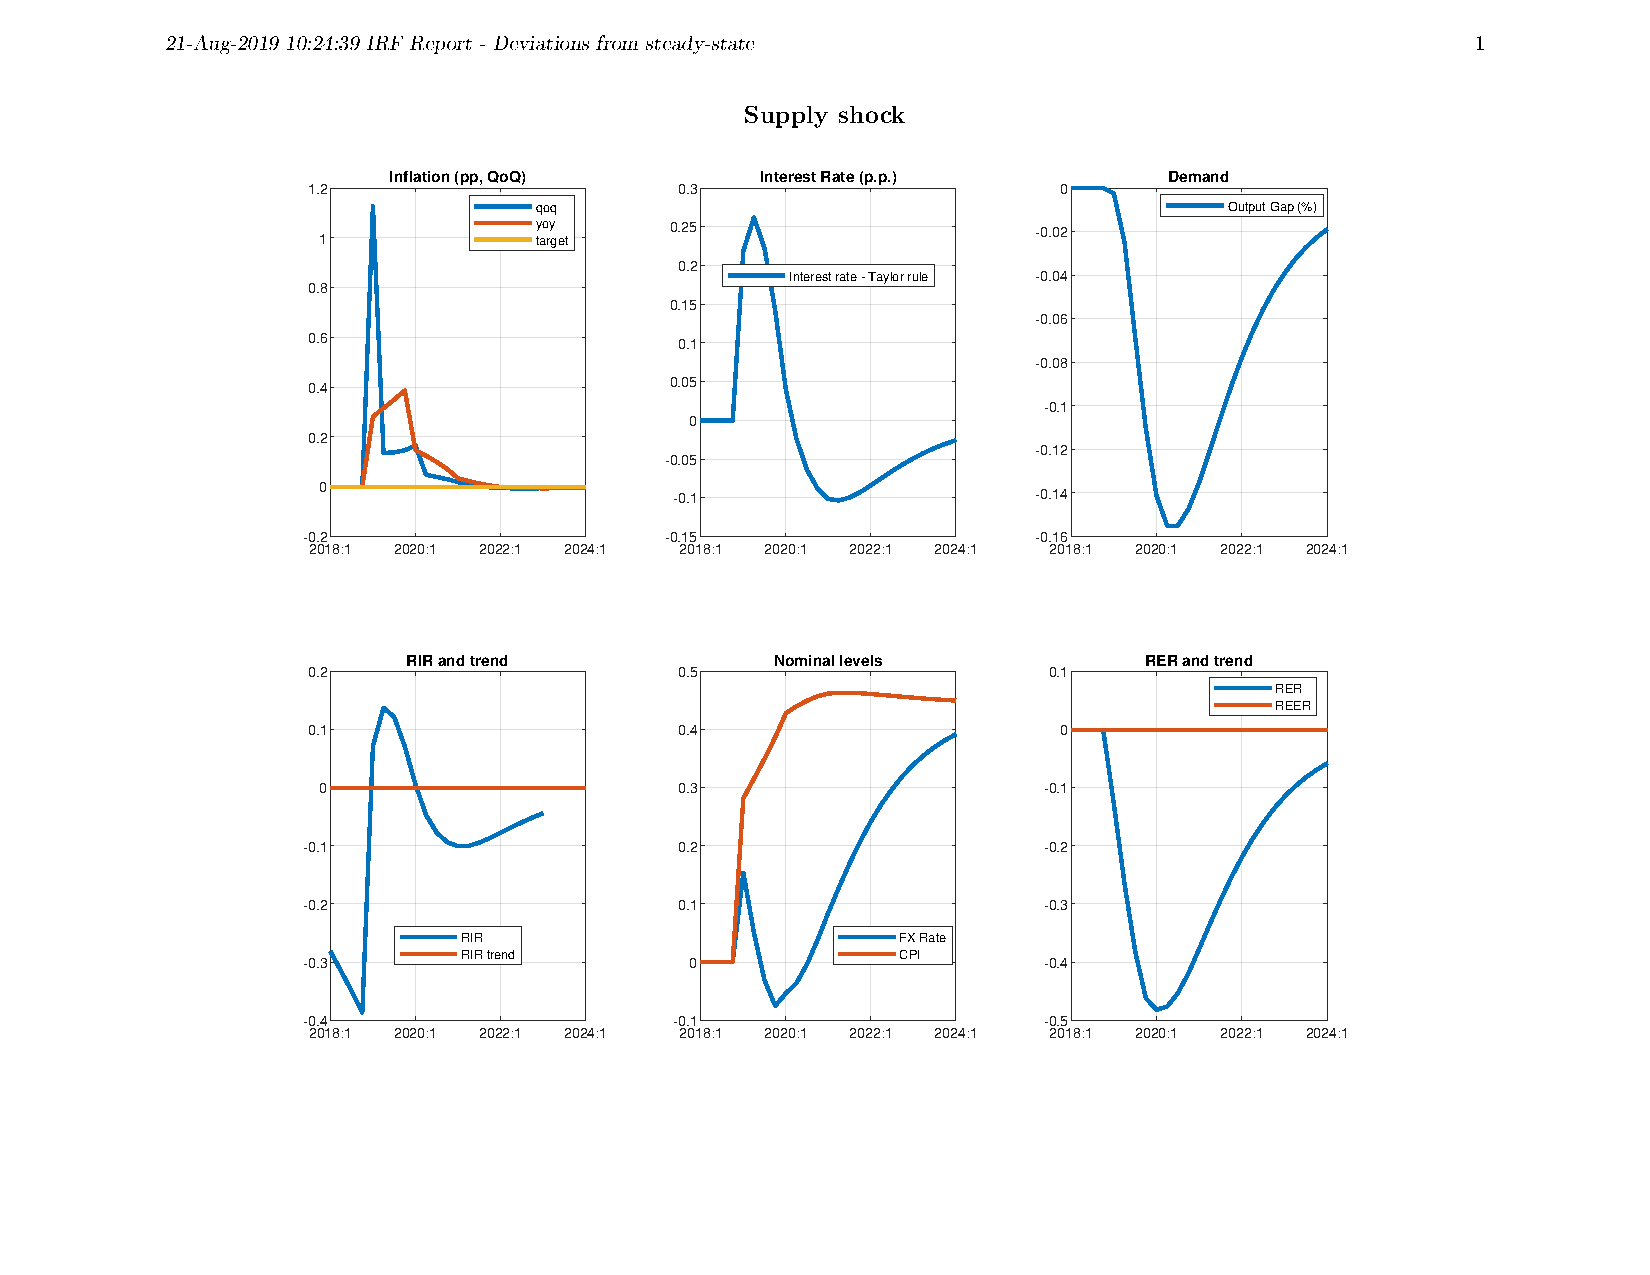
\includepdf[pages=1,landscape=true,scale=.9,pagecommand={\subsection{Calibrated IRFs}\label{ssec:qpmirfs}},linktodoc=true]{bgpp/reports/irf.pdf}
\includepdf[pages=2-,landscape=true,scale=.9,pagecommand={},linktodoc=true]{bgpp/reports/irf.pdf}

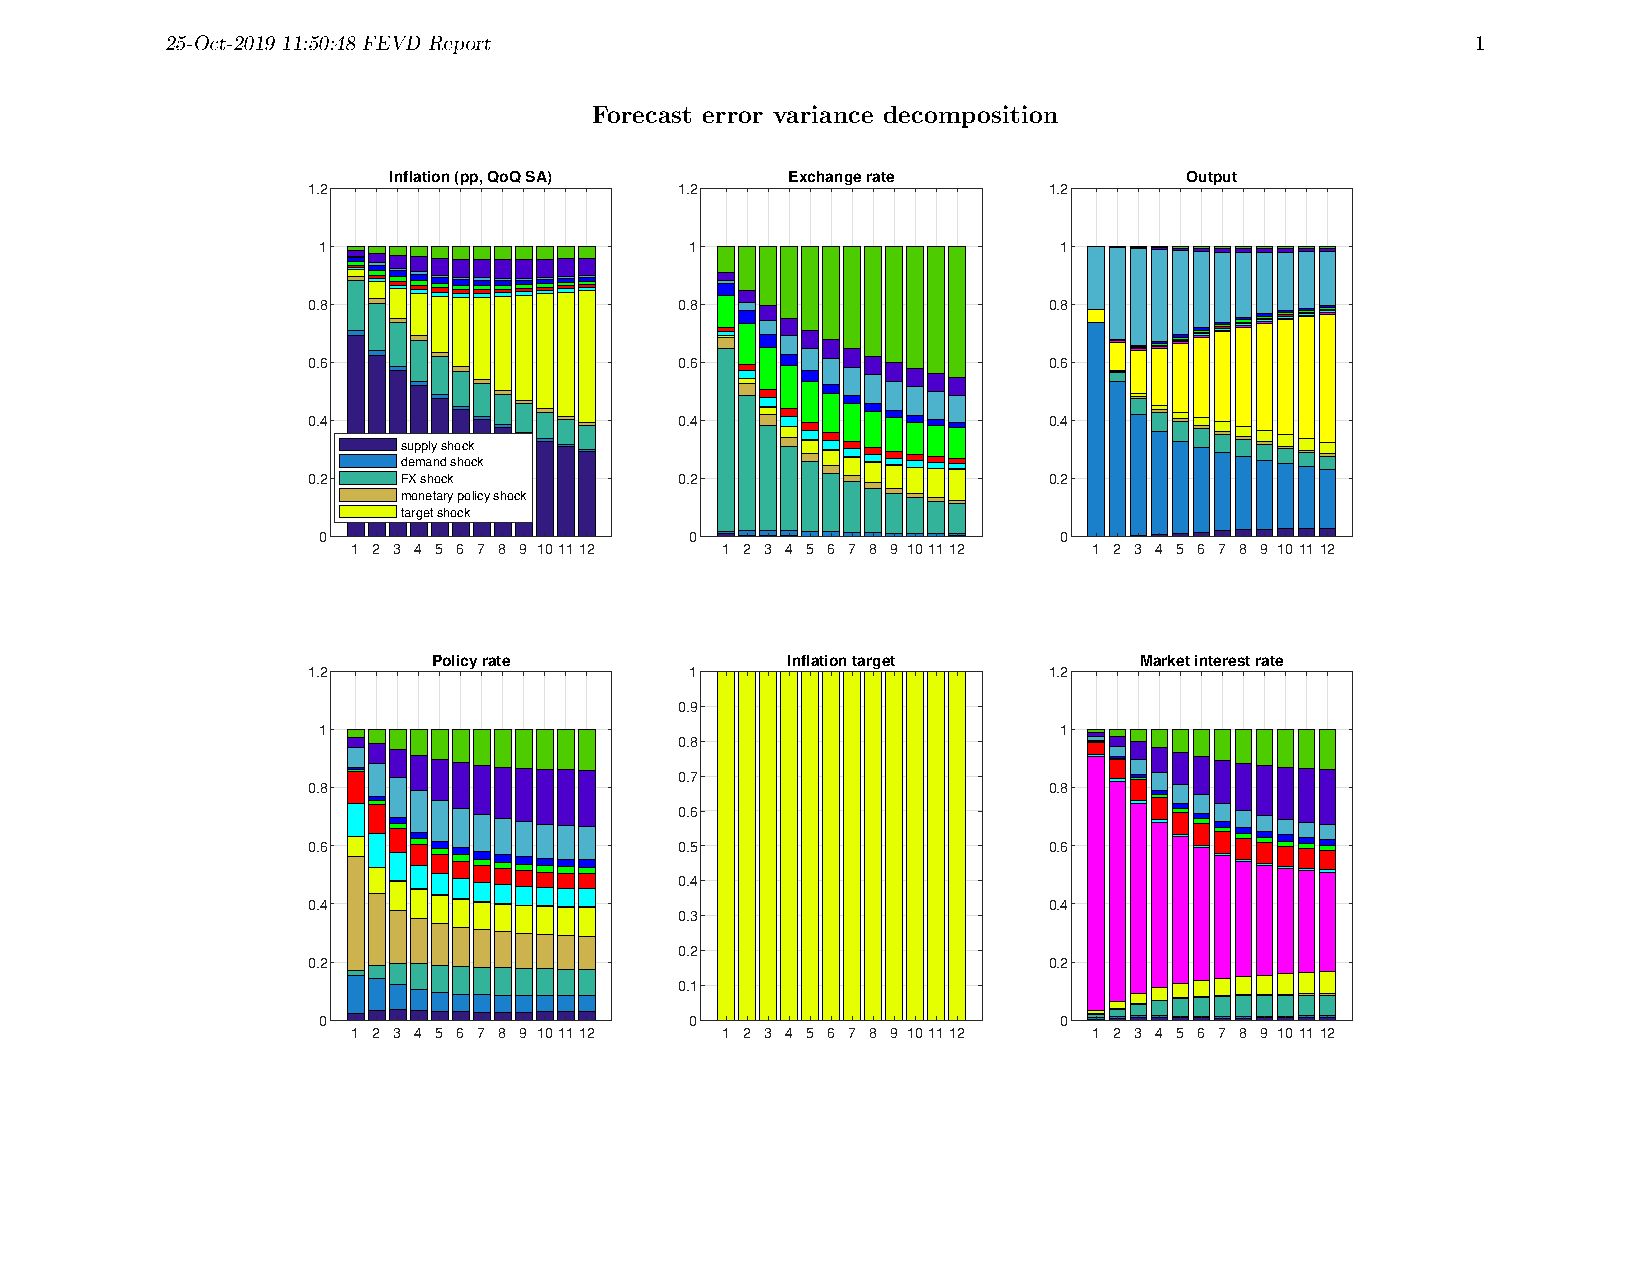
\includepdf[pages=1,landscape=true,scale=.9,pagecommand={\subsection{FEVD}\label{ssec:qpmfevd}},linktodoc=true]{bgpp/reports/fevd.pdf}
\includepdf[pages=2-,landscape=true,scale=.9,pagecommand={},linktodoc=true]{bgpp/reports/fevd.pdf}

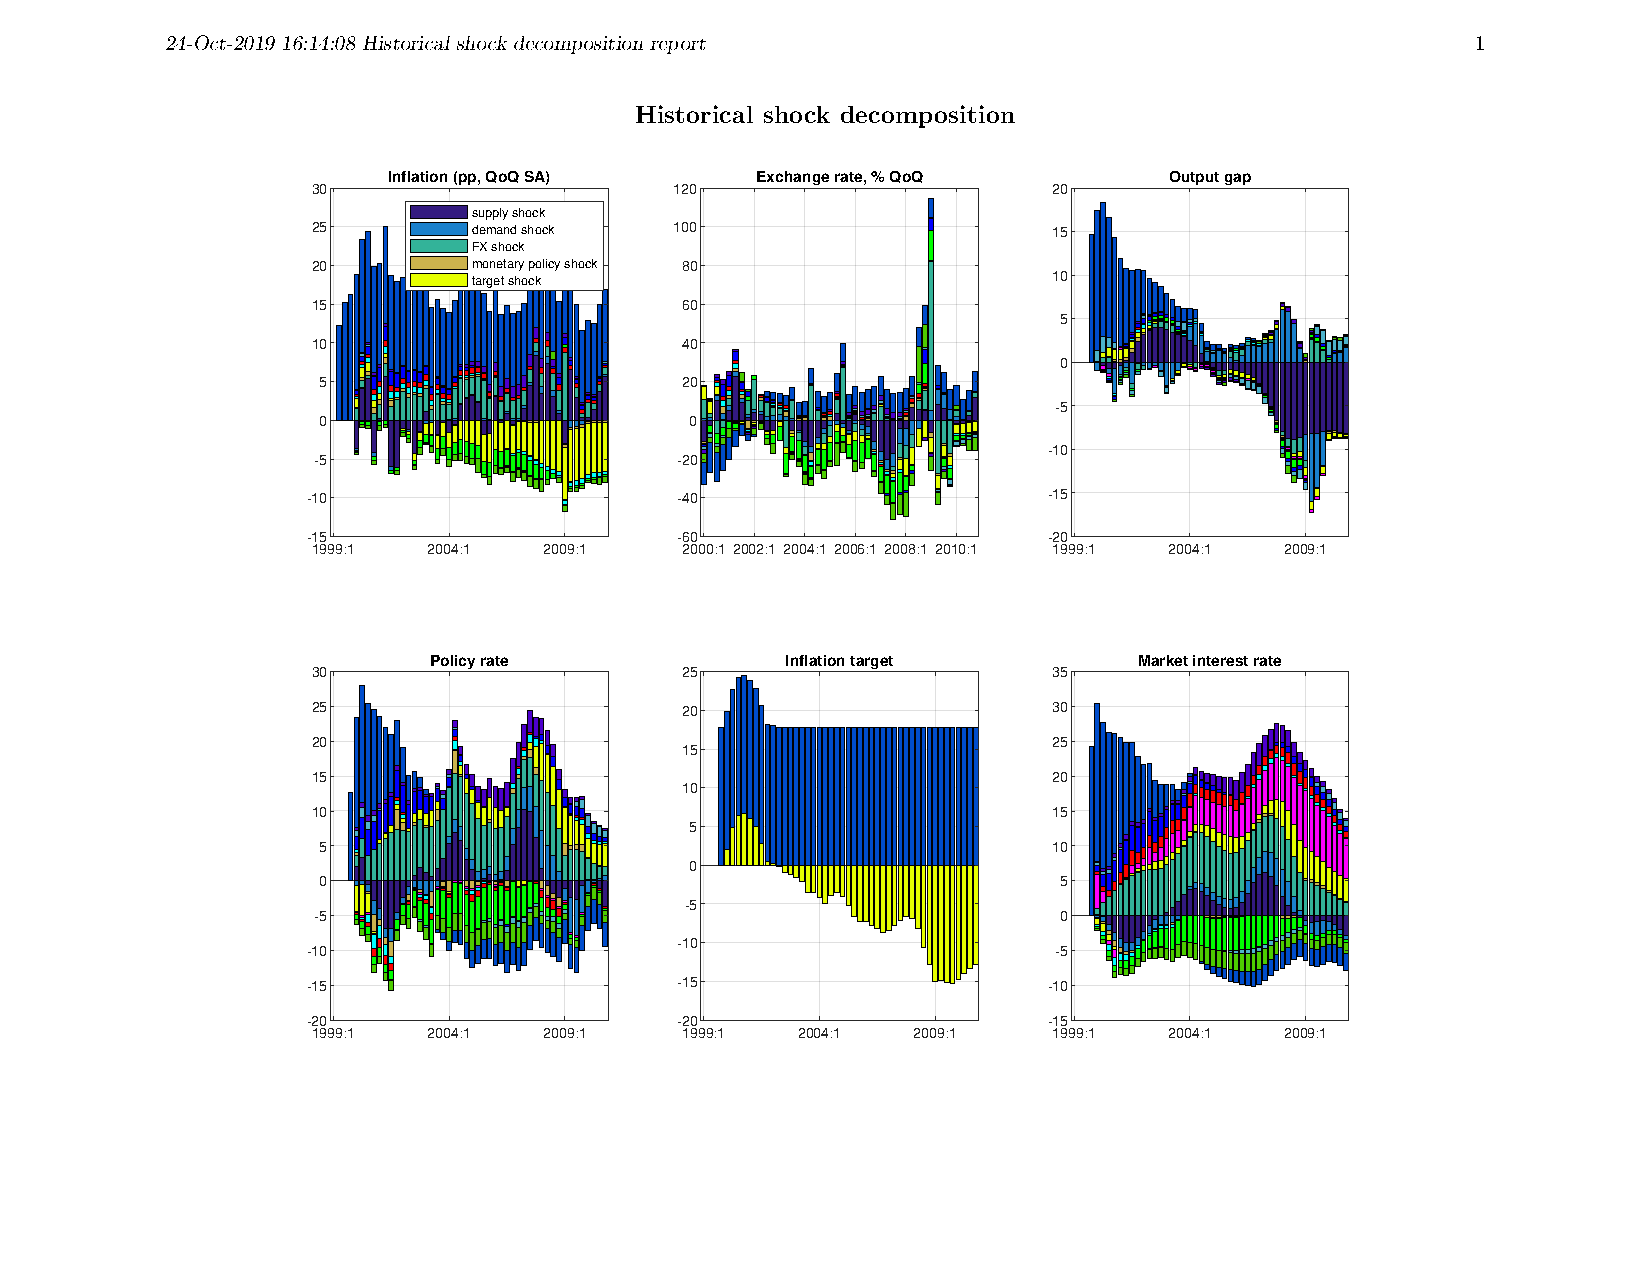
\includepdf[pages=1,landscape=true,scale=.9,pagecommand={\subsection{Historical decomposition: calibrated parameters}\label{ssec:qpmhdecom}},linktodoc=true]{bgpp/reports/hd.pdf}
\includepdf[pages=2-,landscape=true,scale=.9,pagecommand={},linktodoc=true]{bgpp/reports/hd.pdf}


\bibliographystyle{agsm}
\bibliography{bibfile} 

\end{document}



